%%%%%%%%%%%%%%%%%%%%%%%%%%%%%%%%%%%%%%%%%%%%%%%%%%%%%%%%%%%%%%%%%%%
%%% Documento LaTeX 																						%%%
%%%%%%%%%%%%%%%%%%%%%%%%%%%%%%%%%%%%%%%%%%%%%%%%%%%%%%%%%%%%%%%%%%%
% Título:		Capítulo 3
% Autor:  	Ignacio Moreno Doblas
% Fecha:  	2014-02-01
% Versión:	0.5.0
%%%%%%%%%%%%%%%%%%%%%%%%%%%%%%%%%%%%%%%%%%%%%%%%%%%%%%%%%%%%%%%%%%%
\chapterbegin{Plan de pruebas y verificación}
\label{chp:App}
%\minitoc
\section{Funcionamiento de la aplicación}


\section{Precisión de las medidas}
Para cercioranse de que los valores de nivel de presión sonora mostrados en la aplicación se ajustan a la realidad, es necesario comparar los valores para una misma fuente con los obtenidos por un aparato de medición calibrado.

Tras realizar dichas medidas, la aplicación deberá de ser configurada conforme a los resultados obtenidos, introduciendo los parámetros pertinentes en la pantalla dispuesta a dicho efecto.

Dicho proceso es necesario para cada micrófono distinto que sea usado con la aplicación, ya sea por usarla en un teléfono distinto o por utilizar un micrófono externo, ya que las características de cada uno varían, y no puede garantizarse la fidelidad de los resultados de un micrófono con los parámetros de otro.
\subsection{Realización de medidas en laboratorio}
Para las pruebas de calibrado del nivel de presión sonora, se han realizado en el laboratorio medidas de nivel de presión sonora emitido por un monitor de estudio, primero por un sonómetro calibrado, y después por la aplicación.

El sonómetro utilizado ha sido el Svantek SVAN 977.

El micrófono utilizado por la aplicación ha sido el integrado en el teléfono, modelo LG Nexus 5. Según \cite{n5-svcman}, es un micrófono del tipo microelectromecánico, o MEMS según sus siglas en inglés, de la marca Goertek. Sin embargo, la hoja de características del micrófono no está disponible.

Los resultados de la batería de pruebas pueden observarse en la tabla \ref{tab:SAR}. Es notoria la similitud de las mediciones para el tono puro, y un resultado del todo esperado dado que cae dentro del rango de frecuencias típicas de trabajo de un micrófono de un dispositivo móvil.

Sin embargo, cuanto más nos alejamos de dicho funcionamiento típico del micrófono del dispositivo móvil, es posible observar mayores discrepancias. En el límite inferior, se observa cómo la sensibilidad de dicho tipo de micrófonos es limitada, y no es capaz de detectar niveles menores de alrededor de 43 dB.

Presentado ante un ruido blanco, la aplicación reporta un nivel menor que el observado en la lectura del sonómetro. Es de suponer que esto es debido al sonómetro siendo capaz de abarcar un espectro mayor de frecuencias en su medición, y por tanto recibiendo unas lecturas más altas.

\begin{table}[h]%
\centering
\begin{tabular}{|c|c|c|}
    \hline
    \hline
    \tbf{Aparato}&\tbf{Sonómetro} &\tbf{Teléfono}\\ \hline 
    \tbf{Tono 440 Hz} &68.7 dB& 68.6 dB \\ \hline
    \tbf{Fuente sonora apagada}& 37.4 dB& 43.2 dB \\ \hline
    \tbf{Ruido blanco} &  69.3 dB & 62.6 dB\\ \hline
    \tbf{Ruido Rosa} & 69.2 dB& 64.1 dB \\ \hline
    \tbf{Canción}& 63.1 dB & 59.3 dB\\ \hline
    \hline 
\end{tabular}
\caption{Tabla de comparacion de mediciones} \label{tab:SAR}
\end{table} 


\section{Realización de los objectivos}

\subsection{Capacidad de medir la magnitud del ruido ambiente}
La aplicación es capaz de medir la magnitud de ruido ambiente en cualquier momento dado, tan solo hay que comenzar la captación y se muestra un valor estimado en decibelios. Podemos observar que dicho objetivo se cumple en la figura \ref{fig:screen:measure}.
\begin{figure}[h] \centering
    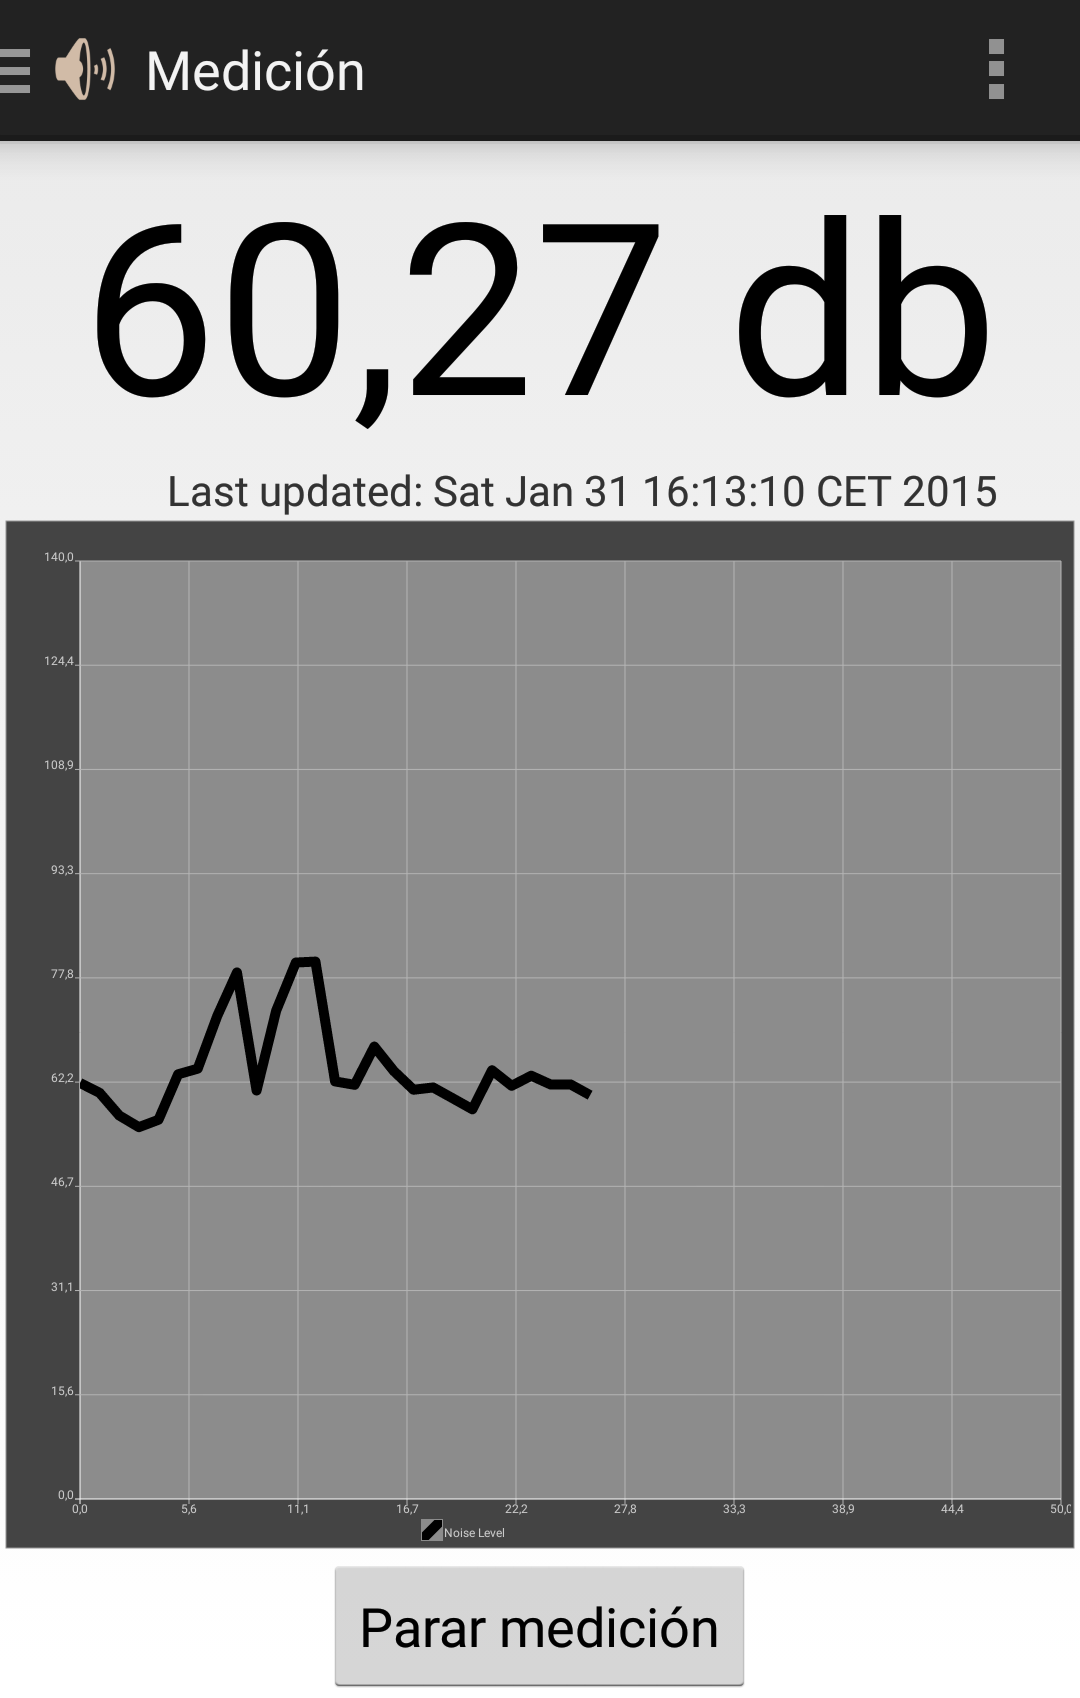
\includegraphics[height=10cm]{graphs/screen_measure.png} \caption{Captura de pantalla de la aplicación mostrando la estimación actual.}\label{fig:screen:measure}
\end{figure}

\subsection{Capacidad de determinar la posición del dispositivo}
La aplicación cumple con el objetivo de ser capaz de determinar la posición absoluta del dispositivo móvil, ya sea dentro del mapa utilizado para representar los datos obtenidos previamente, o durante la operación de recabado de datos. Es posible apreciar cómo el punto azul determina nuestra posición actual en la figura \ref{fig:screen:location}. Durante la medición no se muestra de forma directa la posición absoluta medida, pero es tenida en cuenta en todo momento de la misma.
\begin{figure}[h] \centering
    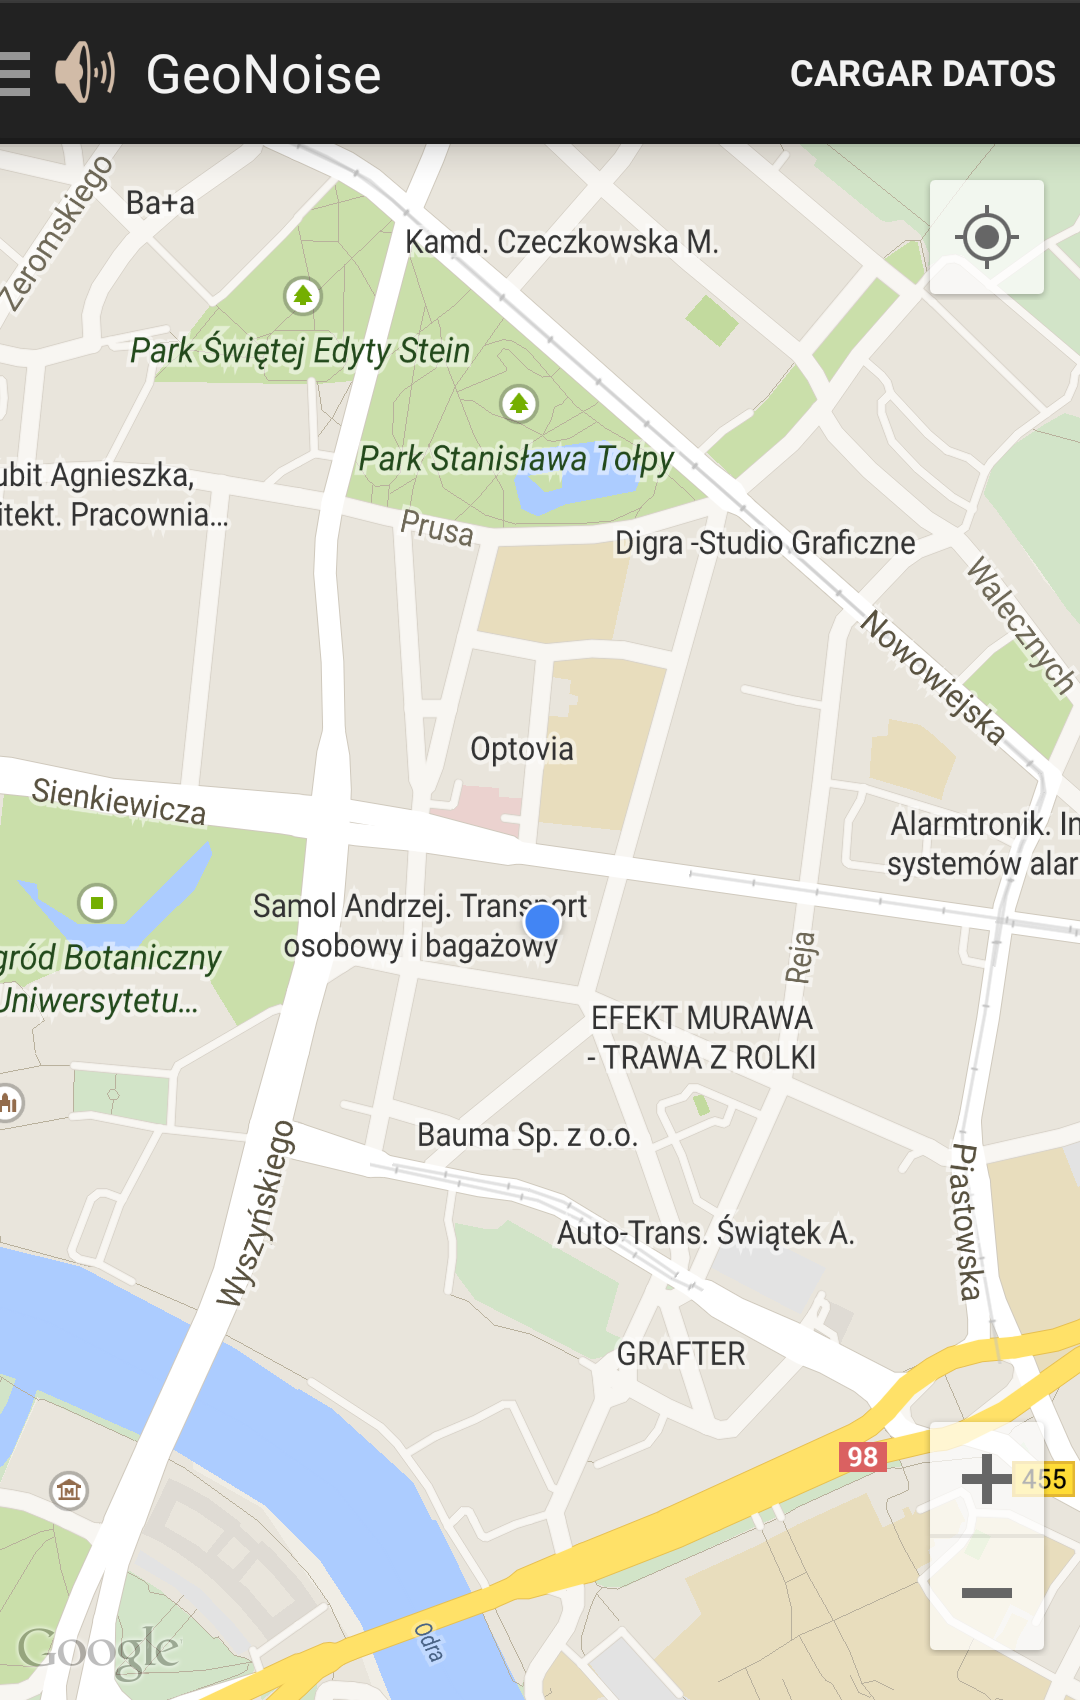
\includegraphics[height=10cm]{graphs/screen_location.png} \caption{Captura de pantalla de la aplicación mostrando la localización actual del dispositivo móvil.}\label{fig:screen:location}
\end{figure}

\subsection{Capacidad de asociar ambas mediciones}
La aplicación vincula en cada operación de muestreo la magnitud medida y la posición absoluta medida, de manera que sea posible conocer a qué punto geográfico pertenece cada medida. Es posible observar dicha asociación en el contenido del archivo creado por cada sesión de grabación, como puede observarse en la figura \ref{fig:dump:file}.

\begin{figure}[h] \centering
\begin{boxedverbatim}
"magnitude","latitude","longitude","accuracy","timestamp"
"62.09779","51.1157184","17.0541213","12.618","31/01/2015 04:13:03"
"60.62046","51.1157184","17.0541213","12.618","31/01/2015 04:13:03"
"57.23939","51.1157184","17.0541213","12.618","31/01/2015 04:13:03"
"55.49906","51.1157184","17.0541213","12.618","31/01/2015 04:13:03"
"56.60217","51.1157184","17.0541213","12.618","31/01/2015 04:13:03"
"63.38877","51.1157184","17.0541213","12.618","31/01/2015 04:13:03"
"64.22864","51.1157184","17.0541213","12.618","31/01/2015 04:13:03"
"72.13268","51.1157184","17.0541213","12.618","31/01/2015 04:13:03"
"78.58884","51.1157184","17.0541213","12.618","31/01/2015 04:13:03"
\end{boxedverbatim}
\caption{Extracto de un archivo CSV producido por la aplicación}
\label{fig:dump:file}
\end{figure}
\subsection{Capacidad de almacenar los datos obtenidos}
Los datos son almacenados inmediatamente después de la finalización de la sesión de grabado a la memoria del dispositivo. Estos pueden ser recuperados conectando el dispositivo móvil a un ordenador personal, o bien representados dentro de la propia aplicación. Una muestra del contenido de un archivo de almacenamiento se puede observar en la figura \ref{fig:dump:file}.

\subsection{Capacidad de mostrar los datos obtenidos sobre un mapa}
Una vez finalizada una sesión de grabación, la aplicación está capacitada para mostrar un listado de las sesiones finalizadas. Una vez seleccionada la sesión que se quiere representar sobre el mapa, la pantalla se actualiza mostrando los datos pertinentes, tal y como se aprecia en la figura \ref{fig:screen:heatmap}.

\begin{figure}[h] \centering
    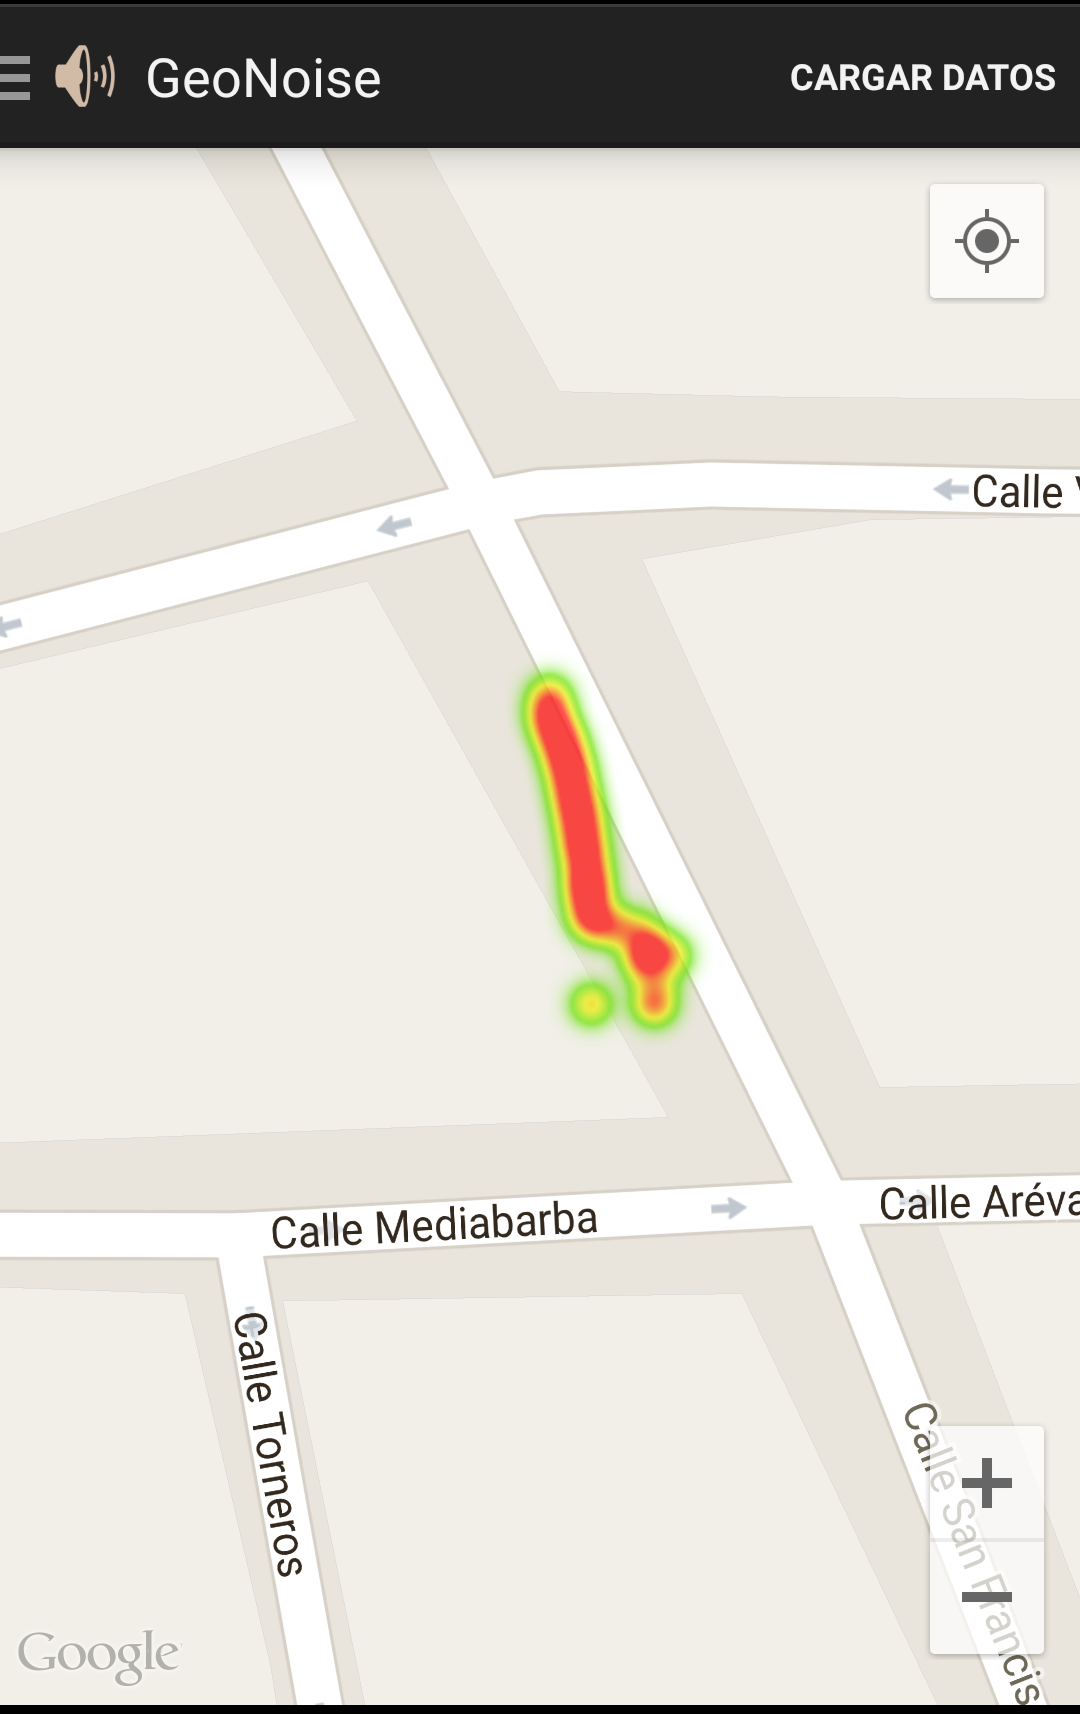
\includegraphics[height=10cm]{graphs/screen_heatmap.png} \caption{Captura de pantalla de la aplicación mostrando la representación de una sesión sencilla de grabación sobre un mapa.}\label{fig:screen:heatmap}
\end{figure}


\chapterend{}